\section{Test-Driven Development (TDD)}

TDD er en udviklignsmetode hvor man skriver sine test \textbf{først}, ser denne test fejle. Derefter implementeres den mindst mulige funktionalitet til at få testen til gå godt.

\begin{figure}[h]
\centering
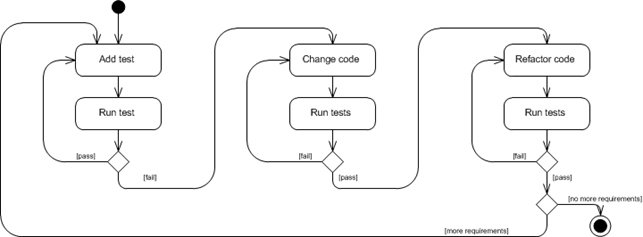
\includegraphics[width=\linewidth]{figs/tdd}
\caption{Red-Green-Refactor mamtra med TDD.}
\label{fig:tdd}
\end{figure}

\subsection{Feature list}
En \textit{feature list} indeholder (pudsigt nok) features, som ønskes implementeret. Herefter udvikler man bare én feature af gangen. \textit{Feature listen} skal indeholde en beskrivelse samt et sæt af test for den pågældende feature.

\subsection{Red-Green-Refactor}
\derp